\section{A Controlled World--Action Design Space}
\label{sec:method}

The study varies an encoder $E_\alpha$, a future representation $Z_\beta$, and a
world--action organization $I_\gamma$. Their configuration is
$c=(\alpha,\beta,\gamma)$, with a shared observation and action interface.
Figure~\ref{fig:architecture} separates these design axes from the common
physical-time protocol. The initial reference configuration provides a comparison
base; it is not a final architecture selection.

\begin{figure*}[t]
\centering
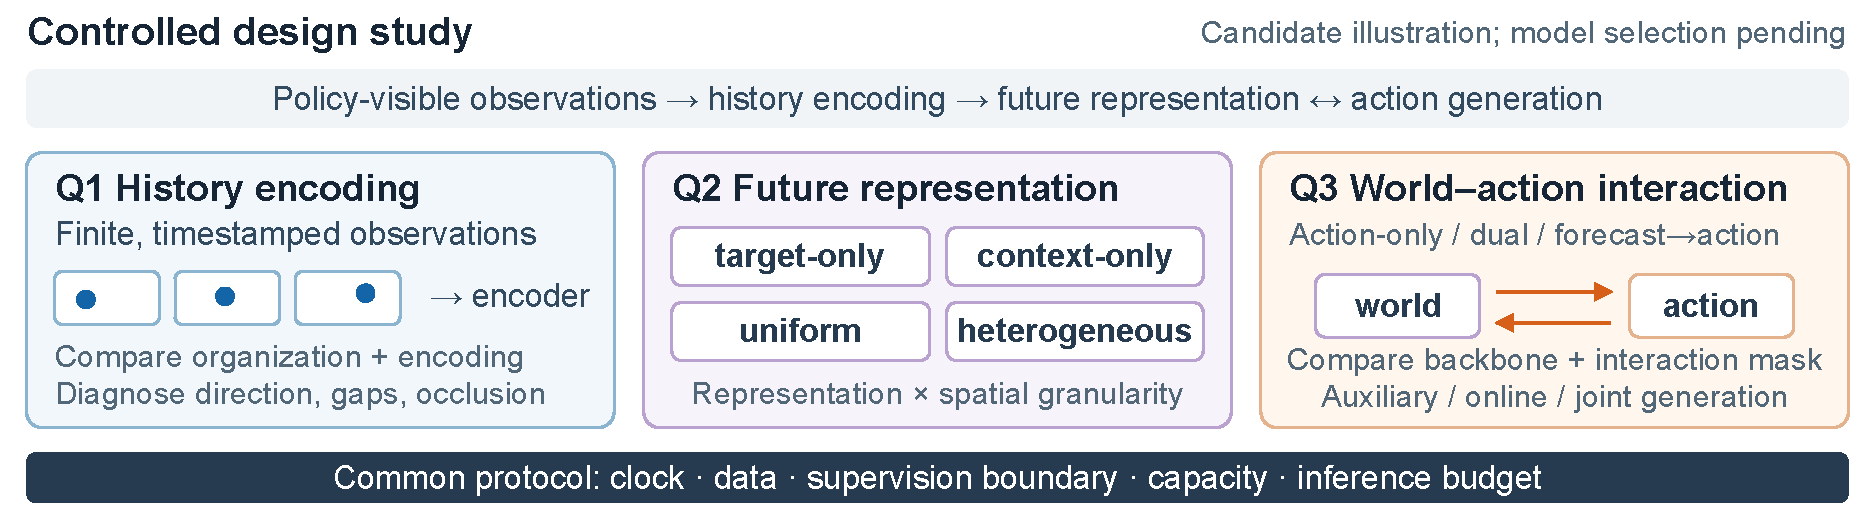
\includegraphics[width=\textwidth]{study_design.pdf}
\caption{The three-axis design study. Q1 changes the encoding of available
history, Q2 changes the future variables and their granularity, and Q3 changes
backbone organization and world--action information flow. Common inputs, physical
times, and budgets define each comparison. Arrows describe conceptual interfaces;
the depicted choices are candidates, not a selected model or measured result.}
\label{fig:architecture}
\end{figure*}

\subsection{Q1: Encoding Finite History}
The encoder maps a finite support of observations to scene and motion tokens:
$\bm X_t=E_\alpha(\mathcal H_t)$. Candidate encodings include RGB history,
time-aware flow, sparse point trajectories, object or scene states, and recurrent
geometric memory. Each specifies coordinate frame, sampling interval, camera
motion, visibility, and early-history validity. Raw displacement without elapsed
time is not a velocity representation. Methods either share the available
history support and token budget or explicitly report the difference. Object
pose and kinematics provided by GT are separate information conditions.
Q1 is evaluated with a stated reference future target and interaction; its
ranking is revisited after Q2 changes what history must support.

An encoding comparison separates access to information from its organization.
One contrast keeps the physical history window fixed while changing the token
representation; another varies the window within the same encoder. They answer
different questions and are not pooled. Flow and trajectories are expressed
relative to declared frames with their true time intervals. Camera-induced
motion must be accounted for or explicitly retained as part of the input.
An early episode with fewer valid observations does not gain synthetic evidence
by repeating its reset frame. A current-object-GT control and a history-object-GT
control hold the remaining robot-state history common, so that their contrast
concerns object information rather than an undeclared change in proprioception.

\subsection{Q2: Future Variables and Granularity}
Given the same available history and execution times, a future predictor forms
\begin{equation}
\hat Z_{\beta,t}=F_\beta(\bm X_t,\{\tau_h^\star\}_{h=0}^{H-1}).
\label{eq:future_interface}
\end{equation}
The target may be rigid pose, trajectory or contact geometry; task-relevant
context may include obstacles, support, moving receptacles, and visibility.
Context is defined by its possible effect on contact, reachability, or collision,
not by a fixed foreground/background split. Static geometry may matter, whereas
unrelated motion need not be predicted.

The comparison distinguishes no future, target-only, context-only, uniform
granularity, and heterogeneous granularity. Representation families such as
RGB or latent state, point trajectories, scene flow, and target \se are
candidates within these roles. A granularity comparison states its region
allocation, spatial and temporal resolution, and decoded-token budget. Changing
both the representation and its budget without a matched control cannot identify
the value of granularity. The action-relevant hypothesis is that preserving
target contact geometry and sufficient contextual constraints may outperform
uniform detail at the same cost; the study also allows the uniform alternative
or auxiliary-only prediction to prevail.

Role and representation are also distinct factors. Comparing target \se with
whole-scene RGB changes both what is described and how it is described. We
therefore record each candidate's target identity source, contextual support,
state variables, spatial allocation, temporal sampling, and prediction budget.
Where the same representation permits it, target-only, context-only, and combined
conditions isolate role coverage. Within a compatible combined representation,
uniform and heterogeneous allocations test granularity while retaining the
same information source and prediction-token allowance. Cross-family comparisons
then report both native prediction error and common action outcomes; a latent
reconstruction loss is not numerically ranked against centimeters of pose error.
These conditional contrasts support a narrower, interpretable conclusion than
a single table in which every row changes role, modality, and cost together.

Temporal resolution is part of granularity. Sampling many future steps at equal
frame intervals can allocate most computation away from the command's execution
window. Each predictor therefore declares the physical horizons it covers and
how the action program queries or pools them. Any extra horizon, adaptive region
selection, or forecast refinement is charged to the same end-to-end budget.
The study can retain a simpler forecast when additional detail is accurate but
does not improve the relevant contact or constraint decision.

For the rigid-target candidate, for example,
\begin{equation}
\hat{\bm T}_h=\Exp(\hat{\bm\xi}_h^\wedge)\hat{\bm T}_t,
\qquad \hat{\bm T}_h\in\se .
\label{eq:se3_prediction}
\end{equation}
This is an output parameterization, not an equivariance claim. Dense displacement
or uncertainty can be added only with its own consumer and evaluation. Predicted
external motion, action-conditioned consequences, and desired task trajectories
are labeled separately. Supplementary Sec.~B gives the inherited \se/flow
candidate mathematics; it does not establish that those heads should survive
model selection.

\subsection{Q3: Backbone Organization and Information Flow}
Q3 compares action-only references, separate world/action systems, prediction
followed by action, and shared or joint world--action organizations. Within a
compatible backbone, interaction masks determine whether action reads future,
future reads action, or both streams interact. Each configuration declares the
visible tokens, gradient paths, generation order, and inference cost; a shared
name does not make two information budgets identical.

Component controls then distinguish auxiliary prediction, online future
conditioning, and joint generation. For the conditional subset these include
\begin{equation}
\begin{aligned}
\text{auxiliary: }&p(\bm a\mid\bm X),\quad q(Z\mid\bm X),\\
\text{online: }&p(\bm a\mid\bm X,\hat Z),\\
\text{joint: }&p(\bm a,Z\mid\bm X).
\end{aligned}
\label{eq:paths}
\end{equation}
Stop-gradient and end-to-end variants address training effects within an
applicable online path; they do not replace the backbone study. A compact
one-way bridge is one such candidate, with zero, swap, noise, and oracle
replacement available when its interface permits a valid intervention. Changing
only the future while fixing perception, robot state, and action-source noise
tests use; a useful effect also requires appropriate action outcomes and safety.

\paragraph{Inference program versus training path.}
A forecast-then-act system makes a world output available before its action
query. A joint generator may instead update action and world variables together;
an action-to-world edge can condition a world output on a proposed action without
feeding a corrected future back into that same action. These programs must be
described by their actual update order, not just by an attention-mask diagram.
The comparison records which intermediate quantities exist when a command is
committed and which are available only during training. In a system without
an independently replaceable forecast, a bridge swap is inapplicable. In a
system that does expose one, a swapped future must preserve the declared
interface and reference condition; replacing arbitrary hidden activations
would test a different perturbation. Backbone allocation, stopping gradients,
and removing an online branch are consequently separate contrasts. Q3 reports
their costs and effects without treating any one intervention as a complete
study of world--action organization.

\paragraph{Selection and cross-comparisons.}
Q1, Q2, and Q3 are compared under stated reference choices, retaining competitive
alternatives for selected cross-checks. Training-only choices and model selection
use the designated development split. The final instance is
\placeholder{history / future / interaction selection}; its description
is filled only after the study and cross-comparisons. More accurate forecasts,
training health, or a fast implementation alone do not select a successful
dynamic policy. Detailed losses, normalization, augmentation, and training
records accompany the actual candidates in Supplementary Secs.~B--E.
